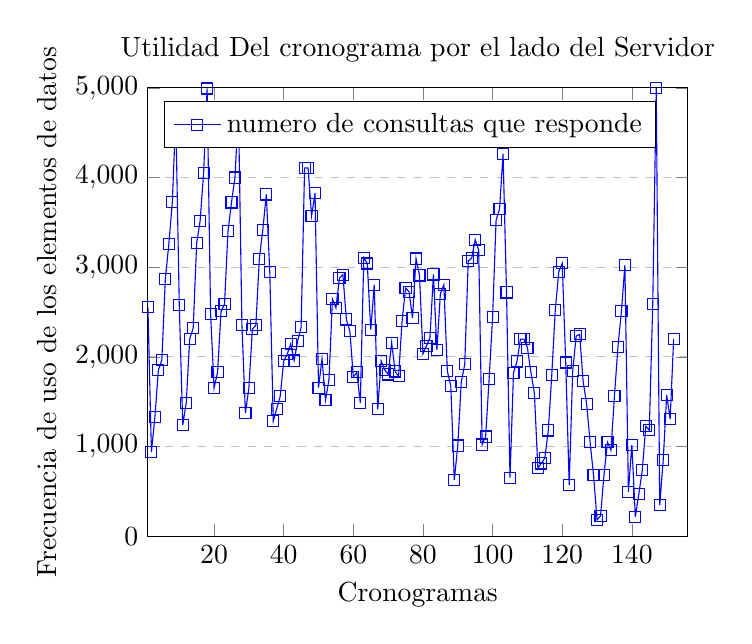
\begin{tikzpicture}
\begin{axis}[
    title={Utilidad Del cronograma por el lado del Servidor},
    xlabel={Cronogramas},
    ylabel={Frecuencia de uso de los elementos de datos},
    xmin=1, xmax=156,
    ymin=0, ymax=5000,
    xtick={},
    ytick={},
    legend pos=north west,
    ymajorgrids=true,
    grid style=dashed,
]

\addplot[
    color=blue,
    mark=square,
    ]
    coordinates {
%UTILIDAD TOTAL
%(cronograma, numero cues que usan al cronograma)
(1,2552)
(2,939)
(3,1329)
(4,1851)
(5,1967)
(6,2867)
(7,3255)
(8,3723)
(9,4693)
(10,2582)
(11,1242)
(12,1485)
(13,2200)
(14,2321)
(15,3267)
(16,3518)
(17,4054)
(18,4993)
(19,2482)
(20,1654)
(21,1827)
(22,2509)
(23,2586)
(24,3401)
(25,3722)
(26,4000)
(27,4770)
(28,2354)
(29,1374)
(30,1654)
(31,2310)
(32,2351)
(33,3095)
(34,3418)
(35,3811)
(36,2946)
(37,1284)
(38,1422)
(39,1561)
(40,1951)
(41,2030)
(42,2144)
(43,1959)
(44,2174)
(45,2332)
(46,4108)
(47,4106)
(48,3574)
(49,3825)
(50,1657)
(51,1978)
(52,1519)
(53,1744)
(54,2644)
(55,2548)
(56,2877)
(57,2917)
(58,2417)
(59,2286)
(60,1776)
(61,1827)
(62,1487)
(63,3106)
(64,3041)
(65,2303)
(66,2802)
(67,1415)
(68,1954)
(69,1856)
(70,1804)
(71,2158)
(72,1837)
(73,1784)
(74,2399)
(75,2769)
(76,2726)
(77,2434)
(78,3096)
(79,2908)
(80,2033)
(81,2122)
(82,2212)
(83,2919)
(84,2075)
(85,2705)
(86,2802)
(87,1840)
(88,1673)
(89,627)
(90,1011)
(91,1719)
(92,1917)
(93,3071)
(94,3100)
(95,3307)
(96,3189)
(97,1022)
(98,1111)
(99,1753)
(100,2445)
(101,3524)
(102,3651)
(103,4266)
(104,2718)
(105,653)
(106,1822)
(107,1949)
(108,2196)
(109,2198)
(110,2103)
(111,1827)
(112,1596)
(113,761)
(114,811)
(115,871)
(116,1179)
(117,1801)
(118,2522)
(119,2947)
(120,3043)
(121,1937)
(122,570)
(123,1838)
(124,2231)
(125,2251)
(126,1729)
(127,1476)
(128,1050)
(129,678)
(130,183)
(131,226)
(132,686)
(133,1048)
(134,960)
(135,1566)
(136,2110)
(137,2508)
(138,3023)
(139,495)
(140,1018)
(141,216)
(142,470)
(143,736)
(144,1226)
(145,1182)
(146,2594)
(147,5000)
(148,347)
(149,847)
(150,1574)
(151,1306)
(152,2200)
    };
    \legend{numero de consultas que responde}

\end{axis}
\end{tikzpicture}

